\documentclass[10.5pt]{article}
 
\usepackage[margin=1in]{geometry} 
\usepackage{amsmath,amsthm,amssymb,graphicx,mathtools,tikz,forest,float,color}
\graphicspath{{./figs/}}
\usepackage{tabularx}

\usepackage{hyperref}
 \hypersetup{
 colorlinks,
 linkcolor=blue
 }

\usetikzlibrary{positioning}

\newcommand{\n}{\mathbb{N}}
\newcommand{\z}{\mathbb{Z}}
\newcommand{\q}{\mathbb{Q}}
\newcommand{\cx}{\mathbb{C}}
\newcommand{\real}{\mathbb{R}}
\newcommand{\field}{\mathbb{F}}
\newcommand{\ita}[1]{\textit{#1}}
\newcommand{\com}[2]{#1\backslash#2}
\newcommand{\oneton}{\{1,2,3,...,n\}}
\newcommand\idea[1]{\begin{gather*}#1\end{gather*}}
\newcommand\ef{\ita{f} }
\newcommand\eff{\ita{f}}
\newcommand\proofs[1]{\begin{proof}#1\end{proof}}
\newcommand\inv[1]{#1^{-1}}
\newcommand\setb[1]{\{#1\}}
\newcommand\en{\ita{n }}
\newcommand{\vbrack}[1]{\langle #1\rangle}

\newtheorem{theo}{Theorem}
\newenvironment{theorem}[2][Theorem]{\begin{trivlist}
\item[\hskip \labelsep {\bfseries #1}\hskip \labelsep {\bfseries #2.}]}{\end{trivlist}}
\newenvironment{definition}[2][Definition]{\begin{trivlist}
\item[\hskip \labelsep {\bfseries #1}\hskip \labelsep {\bfseries #2.}]}{\end{trivlist}}
\newenvironment{lemma}[2][Lemma]{\begin{trivlist}
\item[\hskip \labelsep {\bfseries #1}\hskip \labelsep {\bfseries #2.}]}{\end{trivlist}}
\newenvironment{exercise}[2][Exercise]{\begin{trivlist}
\item[\hskip \labelsep {\bfseries #1}\hskip \labelsep {\bfseries #2.}]}{\end{trivlist}}
\newenvironment{reflection}[2][Reflection]{\begin{trivlist}
\item[\hskip \labelsep {\bfseries #1}\hskip \labelsep {\bfseries #2.}]}{\end{trivlist}}
\newenvironment{proposition}[2][Proposition]{\begin{trivlist}
\item[\hskip \labelsep {\bfseries #1}\hskip \labelsep {\bfseries #2.}]}{\end{trivlist}}
\newenvironment{corollary}[2][Corollary]{\begin{trivlist}
\item[\hskip \labelsep {\bfseries #1}\hskip \labelsep {\bfseries #2.}]}{\end{trivlist}}



 %++++++++++++++++++++++++++++++++++++++++++++++++++
 %+++++++++++++++++++++++++++++++++++++++++++++++++++
\begin{document}

 
\title{MA2503 \\ Bachelor Mathematics Lecture Notes\\
SemA 2016/17}
\author{Peilin \textsc{WU}
%\\ -Personal Usage- \\ \\City University of Hong Kong\\ \\ MA2503 \\ Linear Algebra \\ \\ Test Time: 13-Dec-2016 18:30-21:30 \\ Test Venue: LT5 \\ Seat Number: 0063
} 
\date{\today}


\maketitle
\tableofcontents

%\pagebreak
\newpage
\section{Linear Equation}
\section{Rectangular System and Echelon Form}
GE: Gaussian elimination; G-J: Gauss-Jordan; $U$: row echelon form; $E_A$: reduced row echelon form.
\begin{table}[H]
\centering
\begin{tabularx}{\textwidth}{X|X}
\hline
Task & Method needed \\ \hline
Determining the rank of $A$ & $A \xrightarrow{GE} U$, rank($A$)= number of pivot in $U$\\
Solving linear system $Ax=b$ & $[A|b]\xrightarrow{GE} [U|c]$ or $[A|b]\xrightarrow{GJ} [E_A|d]$ \\
 & noted: if rank($U$) $\neq$ rank($[U|c]$), then inconsistent system\\
Determining the column relation & $A\xrightarrow{GJ} E_A$\\
Computing the inverse of $A_{n\times n}$ & $[A|I_n]\xrightarrow{GJ} [I_n|A^{-1}]$, noted: if $A$ can not reduce to $I_n$, then $A$ singular\\
Testing whether $A \sim B$ & $A \xrightarrow{GE} U_A$ $B \xrightarrow{GE} U_B$, then compare rank($U_A$) equal to rank($U_B$) or not\\
Testing whether $A \overset{row}{\sim} B$ & $A \xrightarrow{GJ} E_A$ $B \xrightarrow{GJ} E_B$, then check whether $E_A=E_B$\\
Testing whether $A \overset{col}{\sim} B$ & $A^T \xrightarrow{GJ} E_{A^T}$ $B \xrightarrow{GJ} E_{B^T}$, then check whether $E_{A^T}=E_{B^T}$\\
Testing whether $b \in span\{v_1,\cdots,v_n\}$ & $[v_1|\cdots|v_n|b]=[A|b]\xrightarrow{GE} [U|c]$\\
Testing whether $span\{v_1,\cdots ,v_n\}=\mathbb{R}^m$ & $[v_1|\cdots |v_n]=A_{m\times n}\xrightarrow{GE}U$, then check whether $rank(A)=m$\\
Finding the fundamental subspaces of $A_{m\times n}$ & $[A|I_m]\xrightarrow{GE}[U|P]$, then the bases are:\\
~ & $R(A)$: basic columns of $A$\\
~ & $R(A^T)$: nonzero rows of $U$\\
~ & $N(A)$: $h_i$'s in the general solution of $Ax=0$\\
~ & $N(A^T)$: last $m-r$ rows of $P$, where $r=rank(A)$\\
Testing whether $R(A^T)=R(B^T)$ $N(A)=N(B)$ & $A\xrightarrow{G-J}E_A$, $B\xrightarrow{G-J}E_B$, then check whether $E_A=E_B$ (ie. whether $A\overset{row}{\sim}B$)\\
Testing whether $R(A)=R(B)$ $N(A^T)=N(B^T)$ & $A^T\xrightarrow{G-J}E_{A^T}$, $B^T\xrightarrow{G-J}E_{B^{T}}$, then check whether $E_{A^T}=E_{B^T}$ (ie. whether $A\overset{col}{\sim}B$) \\
Testing whether $N(A_{m\times n})={0}$ & $A\xrightarrow{GE}U$, then check whether $rank(A)=n$ \\
Testing whether $N(A_{m\times n})^T={0}$ & $A\xrightarrow{GE}U$, then check whether $rank(A)=m$ \\
Testing whether $span\{a_1,\cdots ,a_n\}=span\{b_1,\cdots ,b_n\}$ in $\mathbb{R}^n$ & $(a_1^T \cdots a_n^T)^T=A_{r\times n}\xrightarrow{G_J}E_A$, $(b_1^T \cdots b_n^T)^T=B_{r\times n}\xrightarrow{G_J}E_B$, then check whether the nonzero rows of $E_A$ and $E_B$ coincide \\
Testing whether $\{v_1,\cdots ,v_n\}$ is linearly independent & $[v_1|\cdots |v_n]=A\xrightarrow{GE}U$, then check whether $rank(A)=n$\\
Finding linear relationship among $\{v_1,\cdots ,v_n\}$ & $[v_1|\cdots |v_n]=A\xrightarrow{G-J}E_A$, then read off the relationships from $E_A$ \\
Find a basis for $span\{v_1,\cdots ,v_n \}$ & $[v_1|\cdots |v_n]=A\xrightarrow{GE}U$, then the basic columns of $A$ form a basis\\
Extending $\{v_1,\cdots ,v_n\}$ $(r<n)$ to a basis for $\mathbb{R}^n$ & $[v_1|\cdots |v_r|e_1|\cdots |e_n]=A\xrightarrow{GE}U$, then the basic columns of $A$ form a basis
\end{tabularx}
\caption{Summary of applications of Gaussian and Gauss-Jordan elimination}
\end{table}
\pagebreak
\section{Matrix Algebra}
\subsection{Addition and Transposition}
\begin{theo}[Symmetries]
~ Let $A$ be an $n\times n$ square matrix:
\begin{itemize}
\item symmetric: $A^T=A$
\item skew-symmetric: $A^T=-A$
\item hermitian: $A^*=A$
\item skew-hermitian: $A^*=-A$
\end{itemize}
\end{theo}

\subsection{Linearity}
\begin{definition}[Linear Function]
~ Suppose that $\mathcal{D}$ and $\mathcal{R}$ are two sets equipped with an addition and a scalar multiplication operation (consider, for example, $\mathcal{D}=\mathbb{C}^n$ and $\mathcal{R}=\mathbb{C}^m$). A function $f$ that maps points in $\mathcal{D}$ to points in $\mathcal{R}$ is said to be a linear function if $f$ satisfies:
$$f(\alpha x+y)=\alpha f(x)+f(y)$$
for all $x,y\in \mathcal{D}$ and all scalars $\alpha $.
\end{definition}

\subsection{Matrix Multiplication}
\begin{definition}[General Definition of Matrix Multiplication]
~ If matrices $A_{m\times p}$ and $B_{p\times n}$ are conformable, the matrix product $AB$ is defined to be the $m\times n$ matrix as following:
$$[AB]_{ij}=A_{i*}B_{*j}=\sum_{k=1}^{p}a_{ik}b_{kj}$$
$$\left(
\begin{array}{cccc}
* & * & \cdots & * \\ 
\vdots & \vdots & ~ & \vdots \\
a_{i1} & a_{i2} & \vdots & a_{ip} \\
\vdots & \vdots & ~ & \vdots \\
* & * & \cdots & * \\ 
    \end{array}
\right)_{m\times p}
\left(
\begin{array}{ccccc}
* & \cdots & b_{1j} & \cdots & * \\ 
* & \cdots & b_{2j} & \cdots & * \\ 
\vdots & ~ & \vdots & ~ & \vdots \\
* & \cdots & b_{pj} & \cdots & * \\ 
    \end{array}
\right)_{p\times n}=
\left(
\begin{array}{ccccc}
* & \cdots & * & \cdots & * \\ 
\vdots & ~ & \vdots & ~ & \vdots \\
* & \cdots & [AB]_{ij} & \cdots & * \\ 
\vdots & ~ & \vdots & ~ & \vdots \\
* & \cdots & * & \cdots & * \\ 
    \end{array}
\right)_{m\times n}$$
\end{definition}
\begin{lemma}[Rows and Columns of a Matrix Product]
~ To express the individual columns and
rows of a matrix product:
\begin{align*}
[AB]_{*j}&=
\left(
\begin{array}{c}
\left[AB\right]_{1j} \\
\left[AB\right]_{2j} \\
\vdots  \\
\left[AB\right]_{mj}
\end{array}
\right)
=\left(
\begin{array}{c}
a_{11}b_{1j}+a_{12}b_{2j}+\cdots +a_{1p}b_{pj} \\ 
a_{21}b_{1j}+a_{22}b_{2j}+\cdots +a_{2p}b_{pj} \\
\vdots \\
a_{m1}b_{1j}+a_{m2}b_{2j}+\cdots +a_{mp}b_{pj} \\
\end{array}
\right)=
\left(
\begin{array}{c}
a_{11}b_{1j} \\ 
a_{21}b_{1j} \\
\vdots \\
a_{m1}b_{1j} \\
\end{array}
\right)+
\cdots+
\left(
\begin{array}{c}
a_{1p}b_{pj} \\ 
a_{2p}b_{pj} \\
\vdots \\
a_{mp}b_{pj} \\
\end{array}
\right)\\
&=A_{*1}b_{1j}+A_{*2}b_{2j}+\cdots +A_{*p}b_{pj}
\end{align*}
\end{lemma}
\subsection{Matrix Inversion}
\begin{definition}[Matrix Inversion]
~ For a given square matrix $A_{n\times n}$, the matrix $B_{n\times n}$ that satisfied the conditions
$$AB=I_n,\qquad BA=I_n$$
is called the inverse of $A$ and is denoted by $B=A^{-1}$. an invertible matrix is said to be nonsingular, and a square matrix with no inverse is called a singular matrix. 
\end{definition}
\begin{theo}[4.\textbf{Characterization of nonsingular matrices}]
~ For an $n\times n$ matrix $A$, the following statements are equivalent:
\begin{itemize}
\item $A^{-1}$ exists ($A$ is nonsingular);
\item $rank(A) = n$;
\item $A \xrightarrow{Gauss-Jordan} I$;
\item $Ax = 0$ has only the trivial solution $x = 0$.
\end{itemize}
\end{theo}
\subsection{Elementary Matrices and Equivalence}
\begin{definition}[Elementary Matrix]
~ Matrices of the form $I-uv^T$ where $u$ and $v$ are $n\times 1$ column vectors with $v^Tu\neq 1$ are called elementary matrices.
\end{definition}
\begin{definition}[Equivalance]
~ whenever $B$ can be derived from $A$ by a combination of elementary row and column operations, we say that $A$ and $B$ are equivalent matrices and write $A \sim B$; in matrix terms,
\begin{align*}
A \sim B &\iff PAQ=B \quad &\textit{for nonsingular }P \textit{ and } Q\\
A \overset{row}{\sim} B &\iff PAQ=B \quad &\textit{for nonsingular }P\\
A \overset{col}{\sim} B &\iff PAQ=B \quad &\textit{for nonsingular }Q
\end{align*}
and note that if $A \overset{row}{\sim} B$, then:
$$B_{*k}=\displaystyle\sum_{j=1}^{n}\alpha_{j}B_{*j} \iff A_{*k}=\displaystyle\sum_{j=1}^{n}\alpha_{j}A_{*j}$$
Same as the column equivalence, in summary, row equivalence preserves column relationships, and column equivalence preserves row relationships.
\end{definition}
\begin{theo}[6.\textbf{Rank Normal Form}]
~ If $A$ is an $m\times n$ matrix such that $rank(A) = r$, then
$$A \sim N_r = 
\begin{pmatrix}
I_r & 0 \\
0 & 0 \\
\end{pmatrix}$$
where $N_r$ is called the rank normal form of $A$. It is the end product of a complete reduction of $A$ by using both row and column operations.
\end{theo}
\begin{theo}[7.\textbf{Testing for equivalence}]
~ For $m\times n$ matrices $A$ and $B$ the following statement are true:
\begin{itemize}
\item $A\sim B \iff rank(A) = rank(B)$ 
\item $A\sim^{row} B \iff E_A = E_B$
\item $A\sim^{col} B \iff E_{A^T} = E_{B^T}$
\end{itemize}
Note: in particular, that:
\begin{itemize}
\item either $A\sim^{row} B$ or $A\sim^{col} B$ implies $A\sim B$, but not vice versa
\item multiplication by nonsingular matrices doesn't change rank.  
\end{itemize}
\end{theo}
\subsection{LU Factorization}
$$PA=LU$$
\textit{Follow the process of Gaussian Elimination.}
$$Ax=b: \quad Ly=b \rightarrow y=Ux$$
\pagebreak
\section{Vector Space}
\begin{theo}[3 \textbf{Characterization of subspaces}]
The range of every linear function $f$: $\mathcal{R}^n \to \mathcal{R}^m$ is a subspace of $\mathcal{R}^m$, and every subspace of $\mathcal{R}^m$ is the range of some linear function $g$: $\mathcal{R}^r \to \mathcal{R}^m$ $(r\leq m)$.
\end{theo}
\begin{theo}[4 \textbf{Testing for equal ranges}]
For $m \times n$ matrices $A$ and $B$ the following statements are true.
\begin{itemize}
\item $R(A^T) = R(B^T)$ if and only if $A \overset{row}{\sim} B$;
\item $R(A) = R(B)$ if and only if $A \overset{col}{\sim} B$.
\end{itemize}
\end{theo}
\begin{theo}[5 \textbf{Testing for equal null spaces}]
For $m \times n$ matrices $A$ and $B$ the following statements are true.
\begin{itemize}
\item $N(A) = N(B)$ if and only if $A \overset{row}{\sim} B$;
\item $N(A^T) = N(B^T)$ if and only if $A \overset{col}{\sim} B$.
\end{itemize}
\end{theo}
\begin{theo}[7 \textbf{Linear independence and rank}]
If $A$ is $m \times n$, then:
\begin{itemize}
\item the columns of $A$ form a linearly independent set if and only if either of the following holds: (i) $N(A) = \{0\}$, or (ii) $rank(A) = n$;
\item the rows of $A$ form a linearly independent set if and only if either of the following holds: (i) $N(A^T) = \{0\}$, or (ii) $rank(A) = m$;
\item if $A$ is a square matrix, then $A$ is nonsingular if and only if:
\begin{itemize}
\item the columns of $A$ form a linearly independent set, or
\item the rows of $A$ form a linearly independent set.
\end{itemize}
\end{itemize}
\end{theo}
\begin{theo}[8 \textbf{Maximal independent subsets}]
if $A$ is an $m\times n$ matrix and $rank(A) = r$, then:
\begin{itemize}
\item any maximal independent subset of columns (rows) from $A$ contains exactly $r$ columns (rows);
\item in particular, the $r$ basic columns in $A$ constitute one maximal independent subset of columns from $A$.
\end{itemize}
\end{theo}
\begin{theo}[9 \textbf{Basic facts of independence}]
For a nonempty set of vectors $\mathcal{S} = \{u_1, u_2,\cdots , u_n\}$ in a space $\mathcal{V}$, the following are true:
\begin{itemize}
\item if $\mathcal{S}$ contains a linearly dependent subset, then $\mathcal{S}$ itself must be linearly dependent; conversely, if $\mathcal{S}$ is linearly independent, then every subset of $\mathcal{S}$ must also be linearly independent;
\item if $\mathcal{S}$ is linearly independent and if $v \in \mathcal{V}$, then the extension set $\mathcal{S}_{ext}=\mathcal{S} \cup \{v\}$ is linearly independent if and only if $v \notin span(\mathcal{S})$;
\item if $\mathcal{S}  \subseteq \mathcal{R}^m$ and if $n > m$, then $\mathcal{S}$ must be linearly dependent.
\end{itemize}
\end{theo}
\begin{theo}[11 \textbf{Characterizations of a basis}]
Let $\mathcal{V}$ be a subspace of $\mathcal{R}^m$, and let $\mathcal{B}=\{b_1,b_2,\cdots ,b_n \}\subseteq \mathcal{V}$. The following statement are equivalent:
\begin{itemize}
\item $\mathcal{B}$ is a basis for $\mathcal{V}$;
\item $\mathcal{B}$ is a minimal spanning set for $\mathcal{V}$;
\item $\mathcal{B}$ is a maximal linearly independent subset of $\mathcal{V}$.
\end{itemize}
\end{theo}
\begin{theo}[12 \textbf{Dimension theorem}]
Let $\mathcal{V}$ be a subspace of $\mathcal{R}^m$. Then any two linearly independent spanning sets (i.e. any two bases) for $\mathcal{V}$ must have the same number of elements.
\end{theo}

\begin{theo}[13 \textbf{Rank plus nullity theorem}]
if $A$ is an $m\times n$ matrix, then:
$$dimR(A)+dimN(A)=n$$
$$dimR(A^T)+dimN(A^T)=m$$
\end{theo}

\begin{theo}[14 \textbf{Dimension of a sum}]
If $\mathcal{X}$ and $\mathcal{Y}$ are subspaces of a vector space $\mathcal{V}$, then:
$$dim(\mathcal{X}+\mathcal{Y})=dim\mathcal{X}+dim\mathcal{Y}-dim(\mathcal{X}\cap \mathcal{Y})$$
\end{theo}
\begin{reflection}[Summary of the rank]
~ if $A$ is an $m\times n$ matrix and $rank(A) = r$, then:
\begin{align*}
r &= \textit{the number of nonzero rows in any row echelon form of }A\\
&= \textit{the number of pivots in any row echelon form of }A\\
&= \textit{the number of basic columns in }A\\
&= \textit{the size of a maximal independent set of columns from }A\\
&= \textit{the size of a maximal independent set of rows from }A\\
&= dim\mathcal{R}(A)\\
&= dim\mathcal{R}(A^T)\\
&= n-dim\mathcal{N}(A)\\
&= m-dim\mathcal{N}(A^T)\\
&= \textit{the size of the largest nonsingular submatrix in }A\\
\end{align*}
\end{reflection}

\begin{figure}[H]
\centering
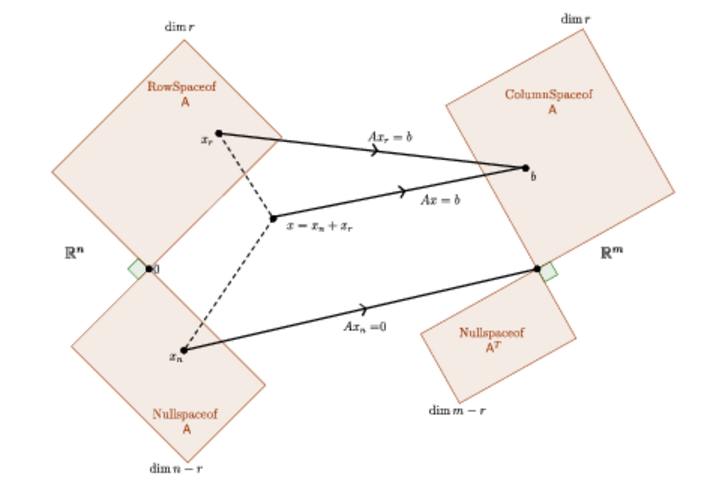
\includegraphics[scale=0.7]{3.PNG}
\caption{Four Fundamental Subspace of Matrix}
\end{figure}
\pagebreak

\begin{figure}[H]
\centering
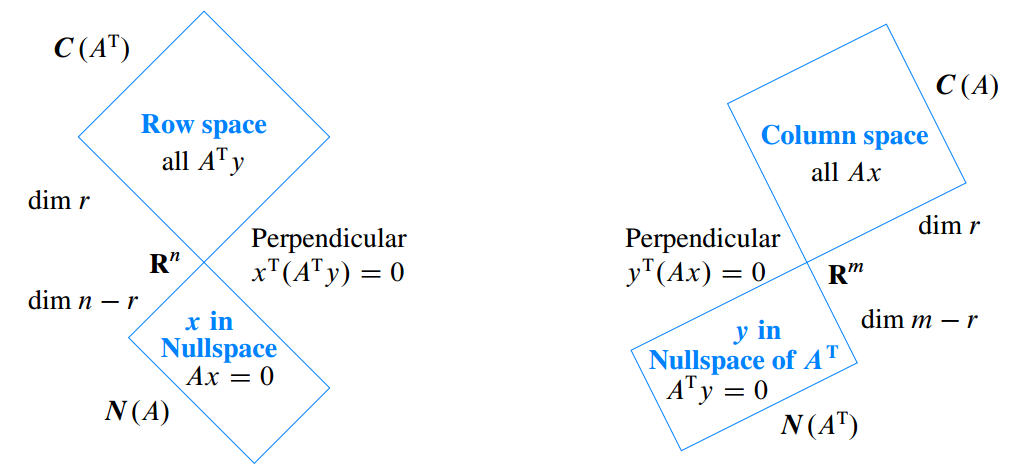
\includegraphics[scale=0.6]{1.PNG}
\caption{Dimensions and orthogonality for any m by n matrix A of rank r}
\end{figure}

\begin{figure}[H]
\centering
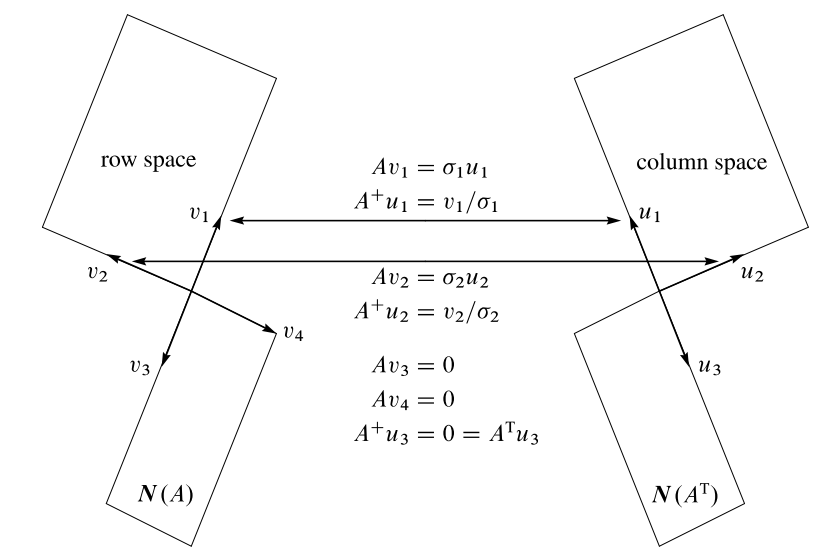
\includegraphics[scale=0.7]{2.PNG}
\caption{Orthonormal bases that diagonalize A (3 by 4) and A$^+$ (4 by 3)}
\end{figure}
\pagebreak

\section{Norms. Inner Product, and Orthogonality}
\begin{definition}[Norm]
~ For an $n \times 1$ vector $x$, the Euclidean norm of $x$ is defined to be:
$$||x||=\left(\sum_{i=1}^{n}x_{i}^{2}\right)^{\frac{1}{2}}=\sqrt{x^Tx}$$
whenever $x\in \mathcal{R}^{n\times 1}$, or
$$||x||=\left(\sum_{i=1}^{n}x_{i}^{2}\right)^{\frac{1}{2}}=\sqrt{x^*x}$$
whenever $x\in \mathcal{C}^{n\times 1}$\\
The $p$-norm can also defined as:
$$||x||_p=\left(\sum_{i=1}^{n}x_{i}^{p}\right)^{\frac{1}{p}}=(x^*x)^{\frac{1}{p}}$$
whenever $x\in \mathcal{C}^{n\times 1}$, $p \geq 1$\\
\end{definition}
\begin{definition}[Standard Inner Product]
~ The Euclidean vector norm can be viewed as a norm induced by the standard inner product:
$$<x,y>=x^Ty=\sum_{i=1}^nx_iy_i \qquad \textit{whenever }x,y\in \mathbb{R}^{n\times 1}$$
$$<x,y>=x^*y=\sum_{i=1}^n\bar{x_i}y_i \qquad \textit{whenever }x,y\in \mathbb{C}^{n\times 1}$$
with the Euclidean norm defined by $||x||=<x,x>^{1/2}$
\end{definition}
\begin{definition}[Orthogonality]
~ Let $\mathcal{V}$ be either $\mathbb{R}^n$ or $\mathbb{C}^n$, Two vectors $x,y\in \mathcal{V}$ are said to be orthogonal (to each other) if $<x,y>=0$, and this is denoted by writing $x\bot y$.\\
And note that:
\begin{itemize}
\item For $\mathbb{R}^n$ with the standard product, $x\bot y \implies x^Ty=0$
\item For $\mathbb{C}^n$ with the standard product, $x\bot y \implies x^*y=0$
\end{itemize}
\end{definition}
\begin{lemma}[General Angle]
~ According to the law of cosine:
$$||u-v||^2=||u||^2+||v||^2-2||u||||v||\cos \theta $$
in general, it implies that:
$$\cos \theta =\dfrac{||u||^2+||v||^2-||u-v||^2}{2||u||||v||}=\dfrac{u^Tv}{||u||||v||}$$
Therefore, the radian measure of the angle between two nonzero vectors $x,y\in \mathbb{R}^n$ is defined to be the number $\theta \in [0,\pi]$ such that:
$$\cos \theta =\dfrac{<x,y>}{||x||||y||}$$
\end{lemma}
\begin{definition}[Orthogonal Set]
~ Let $\mathcal{B}=\{u_1,u_2,\cdots ,u_n\}$ be a set of vectors in $\mathbb{R}^n$ or $\mathbb{C}^n$, $\mathcal{B}$ is called an orthogonal set if $||u_i||=1$ for each $i$ and $u_i \bot u_j$ for all $i\neq j$. In other words, $\mathcal{B}$ is orthogonal if:
\[
 <u_i,u_j> =\delta _{ij} = 
  \begin{cases} 
   1 & \text{if } i = j \\
   0       & \text{if } i \neq j
  \end{cases}
\]
where $\delta _{ij}$ is the classical Kronecker delta symbol.
\end{definition}
\begin{theorem}[Properties of Orthogonal Sets]
~ Let $\mathcal{B}=\{u_1,u_2,\cdots , u_r\}$ be an orthogonal set in $\mathbb{R}^n$($\mathbb{C}^n$), then:
\begin{itemize}
\item $\mathcal{B}$ is linearly independent;
\item if $r=n$, then $\mathcal{B}$ forms an orthogonal basis for the $\mathbb{R}^n$($\mathbb{C}^n$).
\end{itemize}
\end{theorem}
\begin{theorem}[Fourier Expansion]
~ For an orthogonal basis $\mathcal{B}=\{u_1,u_2,\cdots , u_r\}$:
\begin{itemize}
\item the expression:
$$x=\sum_{i=1}^{n}<u_i,x>u_i$$
is called the Fourier expansion of $x$ (with respect to the basis $\mathcal{B}$), and the scalars $\xi _i=<u_i,x>$ are called the Fourier coefficients of $x$.
\item geographically, the Fourier expansion resolves $x$ into $n$ mutually orthogonal vectors $<u_i,x>u_i$, each of which represents the orthogonal projection of $x$ onto the space (line) spanned by $u_i$.
\end{itemize}
\end{theorem}
\begin{theo}[\textbf{Gram-Schmidt Procedure}]
~ The complete Gram-Schmidt procedure proceeds as follows, where $\mathcal{V}=\{\boldsymbol {v}_{1},\boldsymbol {v}_{2},\cdots ,\boldsymbol {v}_{n}\}$, and after the procedure into the orthogonal basis $\mathcal{B}=\{\boldsymbol {\eta }_{1},\boldsymbol {\eta }_{2},\cdots ,\boldsymbol {\eta }_{n}\}$\\
\begin{align*}
\displaystyle {\boldsymbol {\beta }}_{1}&={\boldsymbol {v}}_{1} &\implies \displaystyle {\boldsymbol {\eta }}_{1}&=\boldsymbol {\beta _{1} \over \|{\boldsymbol {\beta }}_{1}\|} \\
\displaystyle {\boldsymbol {\beta }}_{2}&={\boldsymbol {v}}_{2}-\langle {\boldsymbol {v}}_{2},{\boldsymbol {\eta }}_{1}\rangle {\boldsymbol {\eta }}_{1} &\implies \displaystyle {\boldsymbol {\eta }}_{2}&=\boldsymbol {\beta _{2} \over \|{\boldsymbol {\beta }}_{2}\|}\\
\displaystyle {\boldsymbol {\beta }}_{3}&={\boldsymbol {v}}_{3}-\langle {\boldsymbol {v}}_{3},{\boldsymbol {\eta }}_{1}\rangle {\boldsymbol {\eta }}_{1}-\langle {\boldsymbol {v}}_{3},{\boldsymbol {\eta }}_{2}\rangle {\boldsymbol {\eta }}_{2} &\implies \displaystyle {\boldsymbol {\eta }}_{3}&=\boldsymbol {\beta _{3} \over \|{\boldsymbol {\beta }}_{3}\|}\\
&\vdots & ~ &\vdots \\
\displaystyle {\boldsymbol {\beta }}_{k}&={\boldsymbol {v}}_{k}-\sum _{i=1}^{k-1}\langle {\boldsymbol {v}}_{k},{\boldsymbol {\eta }}_{i}\rangle {\boldsymbol {\eta }}_{i} &\implies \displaystyle {\boldsymbol {\eta }}_{k}&=\boldsymbol {\beta _{k} \over \|{\boldsymbol {\beta }}_{k}\|}\\
&\vdots & ~ &\vdots \\
\displaystyle {\boldsymbol {\beta }}_{n}&={\boldsymbol {v}}_{n}-\sum _{i=1}^{n-1}\langle {\boldsymbol {v}}_{n},{\boldsymbol {\eta }}_{i}\rangle {\boldsymbol {\eta }}_{i} &\implies \displaystyle {\boldsymbol {\eta }}_{n}&=\boldsymbol {\beta _{n} \over \|{\boldsymbol {\beta }}_{n}\|}\\
\end{align*}
\end{theo}
\begin{theo}[\textbf{Characteristic of Direct Sums}]
~ Let $\mathcal{V}$ be a vector space and $\mathcal{X}$, $\mathcal{Y}$ be subspaces of $\mathcal{V}$ with respective basis $\mathcal{B}_{\mathcal{X}}$ and $\mathcal{B}_{\mathcal{Y}}$. Then the following statements are equivalent:
\begin{itemize}
\item $\mathcal{V}=\mathcal{X}\oplus \mathcal{Y}$
\item \textit{for each $v\in \mathcal{V}$, there are unique $x\in \mathcal{X}$ and $y\in \mathcal{Y}$, such that $v=x+y$}
\item \textit{$\mathcal{B}_{\mathcal{X}}\cap \mathcal{B}_{\mathcal{Y}}=\emptyset$(empty set) and $\mathcal{B}_{\mathcal{X}}\cup \mathcal{B}_{\mathcal{Y}}$is a basis for $\mathcal{V}$}
\end{itemize}
\end{theo}
\begin{definition}[Orthogonal Complement]
~ Let $\mathcal{V}$ be either $\mathbb{R}^n$ or $\mathbb{C}^n$ and let $\mathcal{M}$ be a subset of $\mathcal{V}$. The orthogonal complement $\mathcal{M}^{\bot}$ of $\mathcal{M}$ is the set of all vectors in $\mathcal{V}$ that are orthogonal to every vector in $\mathcal{M}$. In other words:
$$\mathcal{M}^{\bot}=\{ y\in \mathcal{
V}: <x,y>=0,\forall x\in \mathcal{M}\}$$
\end{definition}
\begin{theo}[\textbf{Orthogonal Complementary Subspaces}]
~ Let $\mathcal{V}$ be either $\mathbb{R}^n$ or $\mathbb{C}^n$. If $\mathcal{M}$ is a subspace of $\mathcal{v}$, then:
$$\mathcal{V}=\mathcal{M}\oplus \mathcal{M}^{\bot}$$
Furthermore, if $\mathcal{N}$ is a subspace such that $\mathcal{V}=\mathcal{M}\oplus \mathcal{M}^{\bot}$ and $\mathcal{N}\bot \mathcal{M}$, then:
$$\mathcal{N}= \mathcal{M}^{\bot}$$
\end{theo}
\begin{theo}[\textbf{Perp Operation}]
~ Let $\mathcal{V}$ be either $\mathbb{R}^n$ or $\mathbb{C}^n$ and let $\mathcal{M}$ be a subset of $\mathcal{V}$. Then the following statements are true:
\begin{itemize}
\item $$dim\mathcal{M}^{\bot}=n-dim\mathcal{M}$$
\item $$(\mathcal{M}^{\bot})^{\bot}=\mathcal{M}$$
\end{itemize}
\end{theo}
\begin{theo}[\textbf{Orthogonal Decomposition Theorem}]
~ For every $A\in \mathbb{R}^{m\times n}$, the following statements are true:
$$\mathcal{R}(A)^{\bot}=\mathcal{N}(A^T)$$
$$\mathcal{N}(A)^{\bot}=\mathcal{R}(A^T)$$
Consequently, every matrix $A\in \mathbb{R}^{m\times n}$ produces an orthogonal decomposition of $\mathbb{R}^m$ and $\mathbb{R}^n$ in th sense that:
$$\mathbb{R}^m=\mathcal{R}(A)\oplus \mathcal{R}(A)^{\bot}=\mathcal{R}(A)\oplus \mathcal{N}(A^T)$$
$$\mathbb{R}^n=\mathcal{N}(A)\oplus \mathcal{N}(A)^{\bot}=\mathcal{N}(A)\oplus \mathcal{R}(A^T)$$
\end{theo}
\pagebreak
\section{Determinants}
\begin{definition}[Determinant]
~ Let $A=[a_{ij}]$ be an $n\times n$ matrix. the determinant of $A$ is defined to be the scalar:
$$det(A)=\sum_{p}\sigma (p)a_{1_{p_{1}}}a_{2_{p_{2}}}\cdots a_{n_{p_{n}}}$$
where the sum is taken over the $n!$ permutations $p=(p_1,p_2,\cdots ,p_n)$ of $(1,2,\cdots ,n)$. The determinant of $A$ can be denoted by $det(A)$ or $|A|$.
\end{definition}
\begin{lemma}[Triangular Determinants]
~ For a triangular matrix, it determinant is equal to the product of its diagonal entries:
$$det(T)=\begin{vmatrix}
t_{11} & t_{12} & \cdots & t_{1n}\\
0 & t_{22} & \cdots & t_{2n}\\
\vdots & \vdots & \ddots & \vdots \\
0 & 0 & \cdots & t_{nn}
\end{vmatrix}=t_{11}t_{22}\cdots t_{nn}$$
\end{lemma}
\begin{theo}[2.\textbf{Effects of row operations}]
~ Let $B$ be the matrix obtained from $A_{n\times n}$ by one of the three elementary row operations:
\begin{itemize}
\item type I: interchange rows $i$ and $j$
\item type II: multiply row $i$ by $\alpha \neq 0$
\item type III: add $\alpha $ times row $i$ to row $j$
\end{itemize}
Then, the determinant $det(B)$ is given by:
\begin{itemize}
\item $det(B)=-det(A)$ for the type I operations
\item $det(B)=\alpha det(A)$ for the type II operations
\item $det(B)=det(A)$ for the type III operations
\end{itemize}
\end{theo}
\begin{theo}[3.\textbf{Invertibility and Determinants}]
~ For every $n\times n$ matrix $A$, the following statements are true:
\begin{itemize}
\item $A$ is nonsingular if and only if $det(A)\neq 0$, or equivalently
\item $A$ is singular if and only if $det(A)=0$
\end{itemize}
\end{theo}
\begin{theo}[4.\textbf{Product Rule}]
~ For all $n\times n$ matrices $A$ and $B$,
$$det(AB)=det(A)det(B)$$
\end{theo}
\begin{definition}[Cofactor Expansion]
~ Let $A$ be an $n\times n$ matrix, with $n\geq 2$. The $(i,j)$-minor of $A$, $M_{ij}$, is defined to be the determinant of the $(n-1)\times (n-1)$ submatrix of $A$ obtained by deleting the $i$-th row and the $j$-th column of $A$. The $(i,j)$-cofactor of $A$, $A_{ij}$, is defined to be $(-1)^{i+j}M_{ij}$. And follow the definition, we can express the determinant as the following:
$$det(A)=a_{i1}A_{i1}+a_{i2}A_{i2}+\cdots +a_{in}A_{in}, \qquad (\textit{about the row }i)$$
$$det(A)=a_{1j}A_{1j}+a_{2j}A_{2j}+\cdots +a_{nj}A_{nj}, \qquad (\textit{about the column }j)$$
\end{definition}
\begin{theorem}[Characteration of Nonsingular Matrices]
~ If $A$ is a $n\times n$ matrix, the the following statement are equivalent:
\begin{itemize}
\item $A^{-1}$n exists ($A$ is nonsingular)
\item $rank(A)=n$
\item $A\xrightarrow{G-J}I$
\item $Ax=0$ has only the trivial solution $x=0$
\item $A$ is the product of elementary matrices of type I, II or III
\item the columns of $A$ forms a linearly independent set
\item the rows of $A$ forms a linearly independent set
\item $det(A)\neq 0$
\end{itemize}
\end{theorem}
\section{Eigenvalue and Eigenvectors}
\begin{definition}[Eigenvalue and Eigenvector]
~ For an $n\times n$ matrix $A$, scalar $\lambda$ and vectors $x_{n\times 1}\neq 0$ satisfying $Ax=\lambda x$ are called the eigenvalue and eigenvectors of $A$, and any pair, $(\lambda ,x)$, is called an eigenpair for $A$. The set of distinct eigenvalues, denoted by $\sigma (A)$, is called the spectrum of $A$.
\end{definition}
\begin{definition}[Similarity Transformation]
~ Two $n\times n$ matrices $A$ and $B$ are said to be similar if there exists a nonsingular matrix $P$ such that $P^{-1}AP=B$. The product $P^{-1}AP$ is called a similarity transformation of $A$.
\end{definition}
\begin{definition}[Diagonalizability]
~ Let A be an $n\times n$ matrix
\begin{itemize}
\item $A$ is said to be diagonalizable if $A$ is similar to a diagonal matrix.
\item $A$ i9s said to have a complete set of eigenvectors if $A$ has a set of $n$ linearly independent eigenvectors, if $A$ fails to process a complete set of eigenvectors, then $A$ is called deficient or defective.
\end{itemize}
\end{definition}
\begin{theo}[4.\textbf{Schur’s triangularization theorem}]
~ Every square matrix is unitarily similar to an upper-triangular matrix. That is, for each $n\times n$ matrix $A$, there exists a unitary matrix $\mathcal{U}$ (not unique) and an upper-triangular matrix $T$ (not unique) such that $\mathcal{U}^*A\mathcal{U} = T$, and the diagonal entries of $T$ are the eigenvalues of $A$.
\end{theo}
\begin{theo}[5.\textbf{The Cayley-Hamilton Theorem}]
~ Every square matrix satisfies its own characteristic equation $p(\lambda )=0$
\end{theo}
\begin{definition}[Multiplicities]
~ Let $\lambda \in \sigma (A)=\{\lambda _1,\lambda _2,\cdots ,\lambda _s\}$
\begin{itemize}
\item The algebraic multiplicity of $\lambda $, denoted by $alg\ mult_{A}(\lambda )$, is the number of times it is repeated as a root of the characteristic polynomial. 
\item when $alg\ mult_{A}(\lambda )=1$, $\lambda $ is called a simple eigenvalue.
\item the geometric multiplicity of $\lambda $, denoted by $geo\ mult_{A}(\lambda )$, is the dimension of the eigenspace $\mathcal{N}(A-\lambda I)$. 
\item Eigenvalues such that $alg\ mult_{A}(\lambda )=geo\ mult_{A}(\lambda )$ are called semisimple eigenvalues of $A$.
\end{itemize}
\end{definition}
\begin{theo}[7.\textbf{Diagonalizality and multiplicities}]
~ An $n\times n$ matrix $A$ is diagonalizable if and only if:
$$geo\ mult_{A}(\lambda )=alg\ mult_{A}(\lambda )$$
for each $\lambda \in \sigma (A)$, i.e. if and only if every eigenvalue is semisimple.
\end{theo}
\pagebreak
\end{document}